\documentclass[12pt]{report}
\usepackage[utf8]{inputenc}
\usepackage[russian]{babel}
%\usepackage[14pt]{extsizes}
\usepackage{listings}
\usepackage{graphicx}
\usepackage{amsmath,amsfonts,amssymb,amsthm,mathtools} 
\usepackage{pgfplots}
\usepackage{filecontents}
\usepackage{indentfirst}
\usepackage{eucal}
\usepackage{enumitem}
\frenchspacing

\usepackage{indentfirst} % Красная строка


\usetikzlibrary{datavisualization}
\usetikzlibrary{datavisualization.formats.functions}

\usepackage{amsmath}




% Для листинга кода:
\lstset{ %
language=C++,                 % выбор языка для подсветки (здесь это С++)
basicstyle=\small\sffamily, % размер и начертание шрифта для подсветки кода
numbers=left,               % где поставить нумерацию строк (слева\справа)
numberstyle=\tiny,           % размер шрифта для номеров строк
stepnumber=1,                   % размер шага между двумя номерами строк
numbersep=5pt,                % как далеко отстоят номера строк от подсвечиваемого кода
showspaces=false,            % показывать или нет пробелы специальными отступами
showstringspaces=false,      % показывать или нет пробелы в строках
showtabs=false,             % показывать или нет табуляцию в строках
frame=single,              % рисовать рамку вокруг кода
tabsize=2,                 % размер табуляции по умолчанию равен 2 пробелам
captionpos=t,              % позиция заголовка вверху [t] или внизу [b] 
breaklines=true,           % автоматически переносить строки (да\нет)
breakatwhitespace=false, % переносить строки только если есть пробел
escapeinside={\#*}{*)}   % если нужно добавить комментарии в коде
}

\usepackage[left=2cm,right=2cm, top=2cm,bottom=2cm,bindingoffset=0cm]{geometry}
% Для измененных титулов глав:
\usepackage{titlesec, blindtext, color} % подключаем нужные пакеты
\definecolor{gray75}{gray}{0.75} % определяем цвет
\newcommand{\hsp}{\hspace{20pt}} % длина линии в 20pt
% titleformat определяет стиль
\titleformat{\chapter}[hang]{\Huge\bfseries}{\thechapter\hsp\textcolor{gray75}{|}\hsp}{0pt}{\Huge\bfseries}


% plot
\usepackage{pgfplots}
\usepackage{filecontents}
\usetikzlibrary{datavisualization}
\usetikzlibrary{datavisualization.formats.functions}

\begin{document}
%\def\chaptername{} % убирает "Глава"
\thispagestyle{empty}
\begin{titlepage}
	\noindent \begin{minipage}{0.15\textwidth}
	
\includegraphics[width=\linewidth]{report_files/bmstu_logo.jpg}
	\end{minipage}
	\noindent\begin{minipage}{0.9\textwidth}\centering
		\textbf{Министерство науки и высшего образования Российской Федерации}\\
		\textbf{Федеральное государственное бюджетное образовательное учреждение высшего образования}\\
		\textbf{~~~«Московский государственный технический университет имени Н.Э.~Баумана}\\
		\textbf{(национальный исследовательский университет)»}\\
		\textbf{(МГТУ им. Н.Э.~Баумана)}
	\end{minipage}
	
	\noindent\rule{18cm}{3pt}
	\newline\newline
	\noindent ФАКУЛЬТЕТ $\underline{\text{«Информатика и системы управления»}}$ \newline\newline
	\noindent КАФЕДРА $\underline{\text{«Программное обеспечение ЭВМ и информационные технологии»}}$\newline\newline\newline\newline\newline
	
	
	\begin{center}
		\noindent\begin{minipage}{1.3\textwidth}\centering
			\Large\textbf{  Отчет по лабораторной работе №3}\newline
			\textbf{по дисциплине "Анализ алгоритмов"}\newline\newline
		\end{minipage}
	\end{center}
	
	\noindent\textbf{Тема} $\underline{\text{Умножение матриц}}$\newline\newline
	\noindent\textbf{Студент} $\underline{\text{Костев Д.И.}}$\newline\newline
	\noindent\textbf{Группа} $\underline{\text{ИУ7-51Б}}$\newline\newline
	\noindent\textbf{Оценка (баллы)} $\underline{\text{~~~~~~~~~~~~~~~~~~~~~~~~~~~}}$\newline\newline
	\noindent\textbf{Преподаватели} $\underline{\text{Волкова Л.Л. }}$\newline\newline\newline
	
	\begin{center}
		\vfill
		Москва~---~\the\year
		~г.
	\end{center}
\end{titlepage}

\setcounter{page}{2}
\tableofcontents

\newpage
\chapter*{Введение}
\addcontentsline{toc}{chapter}{Введение}
Алгоритм Копперсмита — Винограда — алгоритм умножения квадратных матриц, предложенный в 1987 году Д. Копперсмитом и Ш. Виноградом.
В исходной версии асимптотическая сложность алгоритма составляла $O(n^{2,3755})$, где  $n$ — размер стороны матрицы.

Алгоритм Копперсмита — Винограда, с учётом серии улучшений и доработок в последующие годы, обладает лучшей асимптотикой среди известных алгоритмов умножения матриц.

На практике алгоритм Копперсмита — Винограда не используется, так как он имеет очень большую константу пропорциональности и начинает выигрывать в быстродействии у других известных алгоритмов только для матриц, размер которых превышает память современных компьютеров.
Поэтому пользуются алгоритмом Штрассена по причинам простоты реализации и меньшей константе в оценке трудоемкости.

Ниже представлены задачи лабораторной работы.

\begin{enumerate}
	\item Изучение и реализация трёх алгоритмов умножения матриц: обычный, Копперсмита-Винограда, оптимизированный Копперсмита-Винограда.
	\item Сравнительный анализ трудоёмкости алгоритмов на основе теоретических расчетов и выбранной модели вычислений.
	\item Сравнительный анализ алгоритмов на основе экспериментальных данных.
\end{enumerate}

\chapter{Аналитическая часть}
\section{Стандартный алгоритм}

Пусть даны две прямоугольные матрицы
\begin{equation}
	A_{lm} = \begin{pmatrix}
		a_{11} & a_{12} & \ldots & a_{1m}\\
		a_{21} & a_{22} & \ldots & a_{2m}\\
		\vdots & \vdots & \ddots & \vdots\\
		a_{l1} & a_{l2} & \ldots & a_{lm}
	\end{pmatrix},
	\quad
		B_{mn} = \begin{pmatrix}
		b_{11} & b_{12} & \ldots & b_{1n}\\
		b_{21} & b_{22} & \ldots & b_{2n}\\
		\vdots & \vdots & \ddots & \vdots\\
		b_{m1} & b_{m2} & \ldots & b_{mn}
	\end{pmatrix},
\end{equation}

тогда матрица $C$
\begin{equation}
	C_{ln} = \begin{pmatrix}
		c_{11} & c_{12} & \ldots & c_{1n}\\
		c_{21} & c_{22} & \ldots & c_{2n}\\
		\vdots & \vdots & \ddots & \vdots\\
		c_{l1} & c_{l2} & \ldots & c_{ln}
	\end{pmatrix},
\end{equation}

где
\begin{equation}
	\label{eq:M}
	c_{ij} =
		\sum_{r=1}^{m} a_{ir}b_{rj} \quad (i=\overline{1,l}; j=\overline{1,n})
\end{equation}

будет называться произведением матриц $A$ и $B$.
Стандартный алгоритм реализует данную формулу.

\section{Алгоритм Копперсмита -- Винограда}

Если посмотреть на результат умножения двух матриц, то видно, что каждый элемент в нем представляет собой скалярное произведение соответствующих строки и столбца исходных матриц.
Можно заметить также, что такое умножение допускает предварительную обработку, позволяющую часть работы выполнить заранее.

Рассмотрим два вектора $V = (v_1, v_2, v_3, v_4)$ и $W = (w_1, w_2, w_3, w_4)$.
Их скалярное произведение равно: $V \cdot W = v_1w_1 + v_2w_2 + v_3w_3 + v_4w_4$, что эквивалентно (\ref{for:new}):
\begin{equation}
	\label{for:new}
		V \cdot W = (v_1 + w_2)(v_2 + w_1) + (v_3 + w_4)(v_4 + w_3) - v_1v_2 - v_3v_4 - w_1w_2 - w_3w_4.
\end{equation}

Несмотря на то, что второе выражение требует вычисления большего количества операций, чем стандартный алгоритм: вместо четырёх умножений - шесть, а вместо трёх сложений - десять, выражение в правой части последнего равенства допускает предварительную обработку: его части можно вычислить заранее и запомнить для каждой строки первой матрицы и для каждого столбца второй, что позволит для каждого элемента выполнять лишь два умножения и пять сложений, складывая затем только лишь с 2 предварительно посчитанными суммами соседних элементов текущих строк и столбцов.
Из-за того, что операция сложения быстрее операции умножения в ЭВМ, на практике алгоритм должен работать быстрее стандартного.

\section{Оптимизированный алгоритм Копперсмита – Винограда}
Оптимизированный алгоритм Винограда представляет собой обычный алгоритм Винограда, за исключением следующих оптимизаций:
\begin{itemize}
    \item вычисление происходит заранее;
    \item используется битовый сдвиг, вместо деления на 2;
    \item последний цикл для нечётных элементов включён в основной цикл, используя дополнительные операции в случае нечётности.
\end{itemize}

\section{Вывод из аналитической части}
	В данном разделе были рассмотрены алгоритмы классического умножения матриц и алгоритм Винограда, основное отличие которого от классического алгоритма — наличие предварительной обработки, а также количество операций умножения. 
\clearpage

\chapter{Конструкторская часть}

В данном разделе разрабатываются схемы алгоритмов, описанных в аналитическом разделе, а также даётся оценка трудоёмкости этих алгоритмов.
\section{Схемы алгоритмов}

На рисунках  \ref{fig:base}, \ref{fig:grapes} и \ref{fig:grapesOpt} приведены схемы стандартного алгоритма умножения матриц и алгоритма Винограда (обычного и оптимизированного) соответственно. Предполагается, что размеры первой матрицы (n1, m1), а второй - (n2, m2).

Алгоритм Винограда оптимизируется следующим образом.
\begin{enumerate}
\item Cокращается количество умножений в основном цикле и циклах предварительной обработки строк и столбцов.
\item Дополнительный цикл, работающий при нечётном количестве столбцов первой матрицы (строк второй), заменяется на условный оператор, помещённый в основной цикл.
\end{enumerate}

\begin{figure}[h!p]
	\centering
	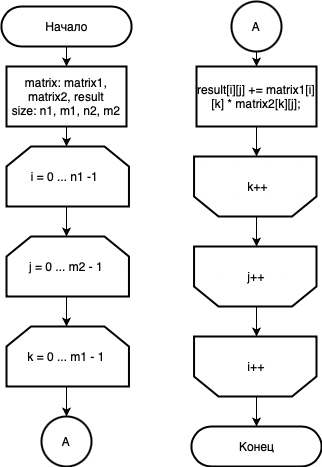
\includegraphics[scale = 0.55]{report_files/base.drawio.png}
	\caption{Схема стандартного алгоритма умножения матриц}
	\label{fig:base}
\end{figure}
\begin{figure}[h!p]
	\centering
	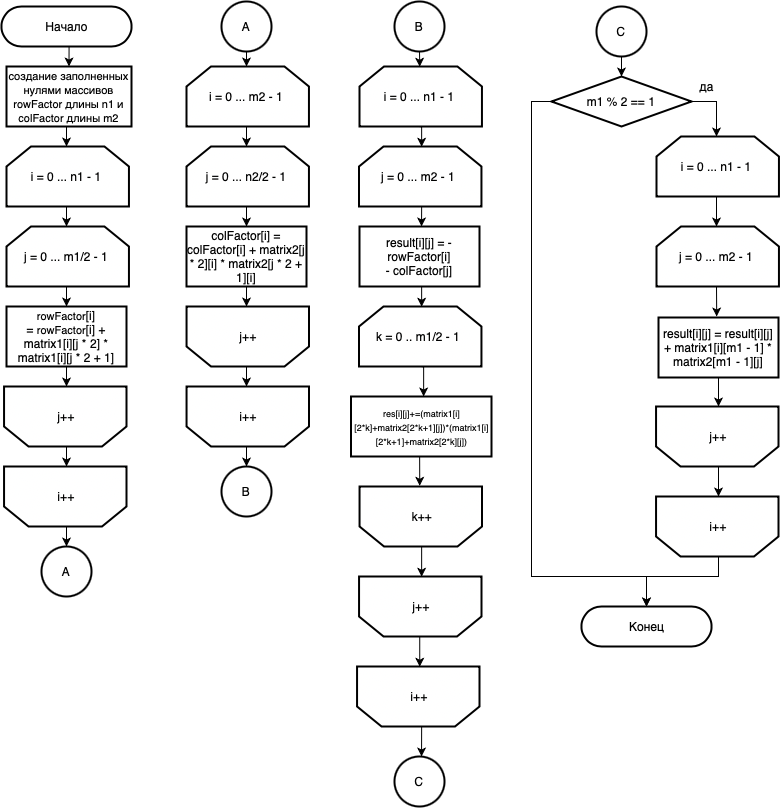
\includegraphics[scale = 0.65]{report_files/vin.drawio.png}
	\caption{Схема алгоритма Винограда}
	\label{fig:grapes}
\end{figure}
\begin{figure}[h!p]\label{vinOptScheme}
	\centering
	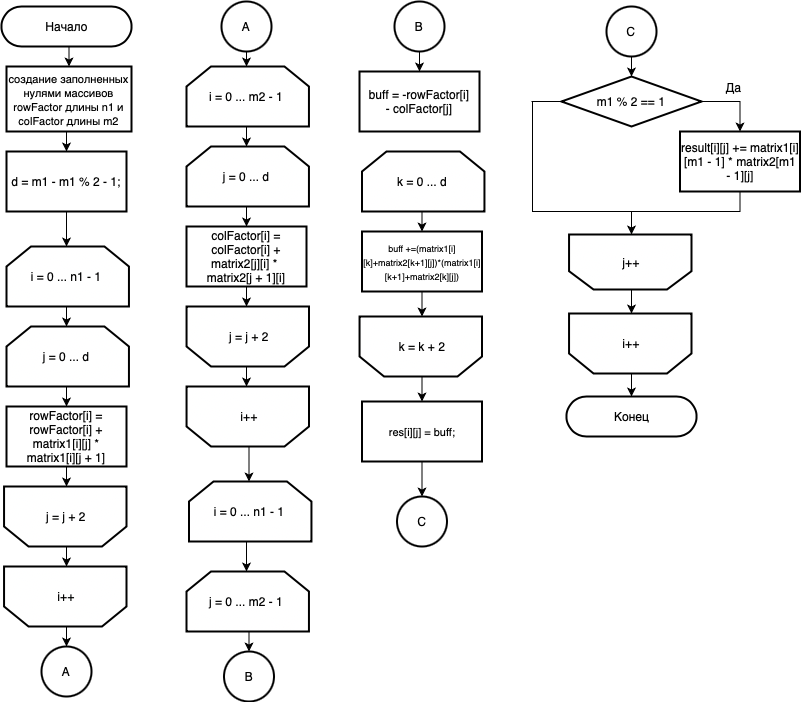
\includegraphics[scale = 0.65]{report_files/vinOpt.drawio.png}
	\caption{Схема оптимизированного алгоритма Винограда}
	\label{fig:grapesOpt}
\end{figure}


\section{Модель вычислений}

Для последующего вычисления трудоемкости введём модель вычислений.

\begin{enumerate}
	\item Операции из списка (\ref{for:opers}) имеют трудоемкость 1.
	\begin{equation}
	\label{for:opers}
	+, -, *, /, \%, ==, !=, <, >, <=, >=, [], ++, {-}-
	\end{equation}
	\item Трудоемкость оператора выбора if условие then A else B рассчитывается, как (\ref{for:if}).
	\begin{equation}
	\label{for:if}
	f_{if} = f_{\text{условия}} +
	\begin{cases}
	f_A, & \text{если условие выполняется,}\\
	f_B, & \text{иначе.}
	\end{cases}
	\end{equation}
	\item Трудоемкость цикла рассчитывается, как (\ref{for:for}).
	\begin{equation}
	\label{for:for}
	f_{for} = f_{\text{инициализации}} + f_{\text{сравнения}} + N(f_{\text{тела}} + f_{\text{инкремента}} + f_{\text{сравнения}})
	\end{equation}
	
	где N - количество итераций цикла.
	\item Трудоемкость вызова функции равна 0.
\end{enumerate}

\section{Трудоёмкость алгоритмов}
Примем, что размеры первой матрицы (r, s), второй - (s, c).
\subsection{Стандартный алгоритм умножения матриц}

Трудоёмкость стандартного алгоритма в выбранной модели вычислений в худшем и лучшем случаях рассчитывается следующим образом:
\begin{equation}
	f_{base} = 2 + r(2 + 2 + c(2 + 2 + s(2 + 11))) = 13scr + 4cr + 4r + 2.
\end{equation}

\subsection{Алгоритм Винограда}
Для алгоритма Винограда худшим случаем являются матрицы с нечётным s, а лучшим - с чётным, из-за того что отпадает необходимость в последнем цикле.

Трудоёмкость алгоритма Винограда является суммой трудоёмкостей следующих последовательно выполненных действий.
\begin{enumerate}
	
	\item Заполнения вектора rowFactor:
	\begin{equation}
	f_{rowFactor} = 3 + r(2 + 2 + \frac{s}{2}(2 + 11)) = 6.5sr + 4r + 3.
	\end{equation}
	
	\item Заполнения вектора colFactor:
	\begin{equation}
	f_{colFactor} = 2 + c(2 + 2 + \frac{s}{2}(2 + 11)) = 6.5sc + 4r + 2.
	\end{equation}
	
	\item Основного цикла заполнения матрицы:
	\begin{equation}
	f_{cycle} = 2 + r(2 + 2 + c(2 + 2 + 7 + \frac{s}{2}(2 + 23))) = 12.5scr + 11cr + 4r + 2.
	\end{equation}
	
	\item Цикла для дополнения умножения, если s нечётный:
	\begin{equation}
	f_{last} = \begin{cases}
	2, & \text{s чётный,}\\
	2 + 2 + r(2 + 2 + c(2 + 13)) = 15cr + 4r + 4, & \text{иначе.}
	\end{cases}
	\end{equation}
\end{enumerate}

Итак, для лучшего случая (s чётный): 
\begin{equation}
f_{vin\_b} = 6.5sr + 4r + 3 + 6.5sc + 4r + 2 + 12.5scr + 11cr + 4r + 2 + 2 = 12.5scr + 6.5sr + 6.5sc + 11cr + 12r + 9.
\end{equation}

Для худшего случая (s нечётный): 
\begin{eqnarray}
f_{vin\_w} = 6.5sr + 4r + 3 + 6.5sc + 4r + 2 + 12.5scr + 11cr + 4r + 2 + 15cr + 4r + 4 =\\ = 12.5scr + 6.5sr + 6.5sc + 26cr + 16r + 11.
\end{eqnarray}

\subsection{Оптимизированный алгоритм Винограда}

Трудоёмкость оптимизированного алгоритма Винограда является суммой трудоёмкостей следующих последовательно выполненных действий.
\begin{enumerate}
	\item Заполнения вектора rowFactor:
	\begin{equation}
	f_{rowFactor} = 5 + r(3 + 2 + \frac{s}{2}(3 + 10)) = 6.5sr + 5r + 5.
	\end{equation}
	
	\item Заполнения вектора colFactor:
	\begin{equation}
	f_{colFactor} = 2 + c(2 + 2 + \frac{s}{2}(2 + 11)) = 6.5sс + 5r + 2.
	\end{equation}
	
	\item Основного цикла заполнения матрицы:
	\begin{equation}
	f_{cycle} = 3 + 2 + r(2 + 2 + c(2 + 2 + 5 + \frac{s}{2}(3 + 15) + f_{last} + 3)) = 9scr + 12cr + f_{last}cr + 4r + 5.
	\end{equation}
	\begin{equation}
	f_{last} = \begin{cases}
	0, & \text{s чётный,}\\
	9, & \text{иначе.}
	\end{cases}
	\end{equation}
\end{enumerate}

Итак, для лучшего случая (s чётный): 
\begin{equation}
f_{vinOpt\_b} = 6.5sr + 5r + 5 + 6.5sс + 5r + 2 + 9scr + 12cr + 4r + 5 = 9scr + 6.5sr + 6.5sc + 12cr + 14r + 12.
\end{equation}

Для худшего случая (s нечётный): 
\begin{equation}
f_{vinOpt\_w} = 6.5sr + 5r + 5 + 6.5sс + 5r + 2 + 9scr + 12cr + 9cr + 4r + 5 = 9scr + 6.5sr + 6.5sc + 21cr + 14r + 12.
\end{equation}

\section{Вывод}
	На основе теоретических данных, полученных из аналитического раздела, были построены схемы алгоритмов умножения матриц, оценены их трудоёмкости в лучшем и худшем случаях.


\chapter{Технологическая часть}

\section{Требование к ПО}

К программе предъявляется ряд требований.

\begin{enumerate}
	\item На вход ПО получает размеры 2 матриц, а также их элементы.
	\item На выходе — ПО печатает матрицу, которая является результатом умножения входных матриц.
\end{enumerate}

\section{Средства реализации}
Для реализации ПО я выбрал язык программирования C++.  

\section{Реализация алгоритмов}

В листингах 3.1 - 3.4 приведена реализация алгоритмов перемножения матриц.

\begin{lstlisting}[label=some-code,caption=Функция умножения матриц обычным способом, language=c++]
Matrix Matrix::convMul(Matrix &matr, clock_t&time)
{
    Matrix result(rows, matr.cols);
    clock_t sTime = clock();
    for (size_t i = 0; i < rows; i++) {
        for (size_t k = 0; k < matr.cols; k++) {
            result.matrix_ptr[i][k] = 0;
            for (size_t j = 0; j < cols; j++)
                result.matrix_ptr[i][k] = result.matrix_ptr[i][k] + matrix_ptr[i][j] * matr.matrix_ptr[j][k];
        }
    }
    clock_t eTime = clock();
    time = eTime - sTime;
    return result;
}
\end{lstlisting}

\begin{lstlisting}[label=some-code,caption=Функция умножения матриц по Винограду,language=c++]
Matrix Matrix::vinogradMul(Matrix &matr, clock_t&time)
{
    Matrix res(rows, matr.cols);
    double *rowFactor = (double *) malloc (rows * sizeof(double));
    double *colFactor = (double *) malloc (matr.cols * sizeof(double ));

    clock_t sTime = clock();
    int d = this->cols / 2;
    for (int i = 0; i < this->rows; i++) {
        rowFactor[i] = matrix_ptr[i][0] * matrix_ptr[i][1];
        for (int j = 1; j < d; j++)
        {
            rowFactor[i] = rowFactor[i] + matrix_ptr[i][2 * j] * matrix_ptr[i][2 * j + 1];

        }
    }

    for (int i = 0; i < matr.cols; i++) {
        colFactor[i] = matr.matrix_ptr[0][i] * matr.matrix_ptr[1][i];
        for (int j = 1; j < d; j++)
        {
            colFactor[i] = colFactor[i] + matr.matrix_ptr[2 * j][i] * matr.matrix_ptr[2 * j + 1][i];
        }
    }

    for (int i = 0; i < this->rows; i++) {
        for (int j = 0; j < matr.cols; j++) {
            res.matrix_ptr[i][j] = -rowFactor[i] - colFactor[j];
            for (int k = 0; k < d; k++)
                res.matrix_ptr[i][j] = res.matrix_ptr[i][j] + (matrix_ptr[i][2 * k] + matr.matrix_ptr[2 * k + 1][j]) *
                                                              (matrix_ptr[i][2 * k + 1] + matr.matrix_ptr[2 * k][j]);
        }
    }

    if (this->cols % 2 == 1)
    {
        for (int i = 0; i < rows; i++)
            for (int j = 0; j < matr.cols; j++)
                res.matrix_ptr[i][j] = res.matrix_ptr[i][j] + matrix_ptr[i][this->cols - 1] *
                                                              matr.matrix_ptr[this->cols - 1][j];
    }
    clock_t eTime = clock();
    time = eTime - sTime;
    free(rowFactor);
    free(colFactor);
    return res;
}
\end{lstlisting}

\begin{lstlisting}[label=some-code,caption=Функция умножения матриц по Винограду с оптимизацией,language=c++]
Matrix Matrix::optimizedMul(Matrix &matr, clock_t&time)
{
    Matrix res(rows, matr.cols);
    double *rowFactor = (double *) malloc (rows * sizeof(double));
    double *colFactor = (double *) malloc (matr.cols * sizeof(double ));

    clock_t sTime = clock();
    int d = cols - cols % 2;
    for (int i = 0; i < this->rows; ++i, ++i) {
        rowFactor[i] = 0;
        for (int j = 0; j < d; ++j, ++j)
            rowFactor[i] = rowFactor[i] + matrix_ptr[i][j] * matrix_ptr[i][j + 1];
    }

    for (int i = 0; i < matr.cols; i++) {
        colFactor[i] = 0;
        for (int j = 0; j < d; ++j, ++j)
        {
            colFactor[i] = colFactor[i] + matr.matrix_ptr[j][i] * matr.matrix_ptr[j + 1][i];
        }
    }

    bool flag = this->cols % 2 == 1;
    double buf;
    for (int i = 0; i < this->rows; ++i) {
        for (int j = 0; j < matr.cols; ++j) {
            buf = -rowFactor[i] - colFactor[j];
            for (int k = 0; k < d; ++k, ++k)
                buf = buf + (matrix_ptr[i][k] + matr.matrix_ptr[k + 1][j]) *
                                                              (matrix_ptr[i][k + 1] + matr.matrix_ptr[k][j]);
            if (flag)
                buf = buf + matrix_ptr[i][this->cols - 1] * matr.matrix_ptr[this->cols - 1][j];
            res.matrix_ptr[i][j] = buf;
        }
    }
    clock_t eTime = clock();
    time = eTime - sTime;
    free(rowFactor);
    free(colFactor);
    return res;
}
\end{lstlisting}

\section{Тестовые данные}

В таблице \ref{tabular:test_rec} приведены тесты для функций, реализующих стандартный алгоритм умножения матриц, алгоритм Винограда и оптимизированный алгоритм Винограда. Все тесты пройдены успешно.

\begin{table}[h!]
	\begin{center}
		\begin{tabular}{c@{\hspace{7mm}}c@{\hspace{7mm}}c@{\hspace{7mm}}c@{\hspace{7mm}}c@{\hspace{7mm}}c@{\hspace{7mm}}}
			\hline
			Первая матрица & Вторая матрица & Ожидаемый результат \\ \hline
			\vspace{4mm}
			$\begin{pmatrix}
			1 & 2 & 3\\
			1 & 2 & 3\\
			1 & 2 & 3
			\end{pmatrix}$ &
			$\begin{pmatrix}
			1 & 2 & 3\\
			1 & 2 & 3\\
			1 & 2 & 3
			\end{pmatrix}$ &
			$\begin{pmatrix}
			6 & 12 & 18\\
			6 & 12 & 18\\
			6 & 12 & 18
			\end{pmatrix}$ \\
			\vspace{2mm}
			\vspace{2mm}
			$\begin{pmatrix}
			1 & 2 & 2\\
			1 & 2 & 2
			\end{pmatrix}$ &
			$\begin{pmatrix}
			1 & 2\\
			1 & 2\\
			1 & 2
			\end{pmatrix}$ &
			$\begin{pmatrix}
			5 & 10\\
			5 & 10
			\end{pmatrix}$ \\
			\vspace{2mm}
			\vspace{2mm}
			$\begin{pmatrix}
			2
			\end{pmatrix}$ &
			$\begin{pmatrix}
			2
			\end{pmatrix}$ &
			$\begin{pmatrix}
			4
			\end{pmatrix}$ \\
			\vspace{2mm}
			\vspace{2mm}
			$\begin{pmatrix}
			1 & -2 & 3\\
			1 & 2 & 3\\
			1 & 2 & 3
			\end{pmatrix}$ &
			$\begin{pmatrix}
			-1 & 2 & 3\\
			1 & 2 & 3\\
			1 & 2 & 3
			\end{pmatrix}$ &
			$\begin{pmatrix}
			0 & 4 & 6\\
			4 & 12 & 18\\
			4 & 12 & 18
			\end{pmatrix}$\\
			\vspace{2mm}
			\vspace{2mm}
		\end{tabular}
	\end{center}
	\caption{\label{tabular:test_rec} Тестирование функций}
\end{table}

\section{Вывод}

В данном разделе были разработаны исходные коды четырёх алгоритмов перемножения матриц: обычный алгоритм, алгоритм с транспонированием, алгоритм Копперсмита — Винограда, оптимизированный алгоритм Копперсмита — Винограда.

\chapter{Исследовательская часть}

\section{Технические характеристики}

Ниже приведеные технические характеристики устройства, на котором было проведенно тестирование ПО.

\begin{itemize}

	\item Операционная система: Windows 11 64-bit.

	\item Оперативная память: 8 ГБ.

	\item Процессор: Intel(R) Core(TM) i5-8250 CPU @ 1.60GHz.

\end{itemize}

\section{Время выполнения алгоритмов}
Время выполнения алгоритм замерялось с помощью применения технологии профайлинга. Данный инстрмуент даёт детальное описание количества вызовов и количества времени CPU, занятого каждой функцией. \newline

В таблицах 4.1 и 4.2 представлены замеры времени работы для каждого из алгоритмов на чётных размерах матриц. Здесь и далее: С — стандартный алгоритм, КВ — алгоритм Копперсмита -- Винограда, ОКВ -- оптимизированный алгоритм Копперсмита -- Винограда.

\begin{table} [h!]
	\caption{Таблица времени выполнения алгоритмов при чётных размерах (в секундах)}
	\begin{center}
		\begin{tabular}{|c c c c|} 
		 	\hline
			Размер матрицы & С & КВ & ОКВ \\  
			\hline
            1000 & 67.20 & 52.30 & 43.50  \\ 
            \hline
            1100 & 76.40 & 56.10 & 47.80  \\ 
            \hline
            1200 & 87.30 & 68.50 & 56.20  \\ 
            \hline
            1300 & 94.90 & 70.80 & 58.20  \\ 
            \hline
            1400 & 102.60 & 76.20 & 63.50  \\ 
            \hline
            1500 & 111.70 & 84.70 & 69.20  \\ 
            \hline
            1600 & 116.40 & 86.60 & 72.70  \\ 
            \hline
            1700 & 128.80 & 93.80 & 82.70  \\ 
            \hline
            1800 & 134.30 & 99.20 & 83.00  \\ 
            \hline
            1900 & 145.60 & 108.00 & 89.20  \\ 
            \hline
            2000 & 154.40 & 120.00 & 96.70  \\ 
            \hline
		\end{tabular}
	\end{center}
\end{table}

\begin{table} [h!]
	\caption{Таблица времени выполнения алгоритмов при нечётных размерах (в наносекундах)}
	\begin{center}
	\begin{tabular}{|c c c c|} 
		\hline
		Размер матрицы & С & КВ & ОКВ \\  
		\hline
        1001 & 70.30 & 53.70 & 43.20  \\ 
        \hline
        1101 & 90.30 & 72.30 & 56.30  \\ 
        \hline
        1201 & 119.00 & 74.70 & 58.80  \\ 
        \hline
        1301 & 95.80 & 70.70 & 62.10  \\ 
        \hline
        1401 & 106.70 & 76.80 & 64.10  \\ 
        \hline
        1501 & 111.90 & 86.00 & 70.10  \\ 
        \hline
        1601 & 118.50 & 88.50 & 77.00  \\ 
        \hline
        1701 & 130.20 & 94.70 & 78.40  \\ 
        \hline
        1801 & 133.40 & 99.50 & 82.70  \\ 
        \hline
        1901 & 145.30 & 111.30 & 89.70  \\ 
        \hline
        2001 & 159.80 & 141.30 & 100.50  \\ 
        \hline
	\end{tabular}
\end{center}
\end{table}


\section{Вывод из исследовательской части}

Реализация умножения матриц с помощью алгоритма Копперсмита -- Винограда в среднем выполняется в 1.3 раза быстрее, чем умножение обычным способом. Учлучшенный алгоритм же работает в 1.5 раз быстрее обычного перемножения и в 1.2 быстрее классического Копперсмита -- Винограда.



\chapter*{Заключение}
\addcontentsline{toc}{chapter}{Заключение}

В рамках данной лабораторной работы были выполнены нижеуказанные задачи.

\begin{enumerate}
	\item Были изучены и реализованы 3 алгоритма перемножения матриц: обычный, Копперсмита -- Винограда, оптимизированный Копперсмита -- Винограда.
	\item Был произведён анализ трудоёмкости алгоритмов на основе теоретических расчётов и выбранной модели вычислений.
	\item Был сделан сравнительный анализ алгоритмов на основе экспериментальных данных.
\end{enumerate}

На основании анализа трудоёмкости алгоритмов в выбранной модели вычислений было показано, что улучшенный алгоритм Винограда имеет меньшую сложность, нежели простой алгоритм перемножения матриц. На основании замеров времени исполнения алгоритмов, был сделан вывод, что алгоритм Копперсмита -- Винограда в среднем в 3.5 раза быстрее чем обычный алгоритм умножения матриц. Кроме этого, я решил добавить в сравнение алгоритм с предварительным транспонированием матрицы. Оказалось, что такая реализация быстрее алгоритма Копперсмита -- Винограда в 1.5 раза и обгоняет классический алгоритм умножения в 3.6 раза. 

\newpage
\addcontentsline{toc}{chapter}{Литература}
\begin{thebibliography}{}
\bibitem{bibKormen}
Кормен Т. Алгоритмы: построение и анализ [Текст] / Корм ен Т. - Вильямс, 2014. - 198 с. - 219 с.
\bibitem{bibGetProcessTimes}
GetProcessTimes function. URL: https://docs.microsoft.com/en-us/windows/win32/api/processthreadsapi/nf-processthreadsapi-getprocesstimes, 01.10.2021
\bibitem{bibwiki}
Алгоритм Копперсмита — Винограда. URL: https://ru.wikipedia.org/wiki/Алгоритм-Копперсмита—Винограда
\end{thebibliography}
	
\bibliographystyle{utf8gost705u}  % стилевой файл для оформления по ГОСТу

\bibliography{51-biblio}          % имя библиографической базы (bib-файла)


\end{document} 